\documentclass[10pt]{sigplanconf}
%\documentclass[letterpaper,10pt]{article}
\usepackage{hyperref}
\usepackage{amsmath,amsthm,amssymb}
%\usepackage[scriptsize,bf]{caption}
%\usepackage{fullpage}
\usepackage{textcomp}
\usepackage{times}
\usepackage{cite}
\usepackage{fancyvrb}
\usepackage{moreverb}
\usepackage{graphicx}
%\usepackage{multicol}

\newcommand{\squishlist}{\begin{list}{$\bullet$}
  {\setlength{\itemsep}{0pt}
    \setlength{\parsep}{3pt}
    \setlength{\topsep}{3pt}
    \setlength{\partopsep}{0pt}
    \setlength{\leftmargin}{1.5em}
    \setlength{\labelwidth}{1em}
    \setlength{\labelsep}{0.5em}
  } }

\newcommand{\squishend}{\end{list}}

\begin{document}

\conferenceinfo{CS7260 2010}{May 5, Atlanta.}
\copyrightyear{2010}
\toappear{Copyright is held by the authors.\\
\textit{CS7260} May 5, Atlanta.}

\title{LRUMAP}
\subtitle{$O(1)$ LRU for Classifying Network Probes}
\authorinfo{Nick Black \and Jolene Tarosky}{Georgia Institute of Technology}{nickblack@linux.com \and jtarosky@gmail.com}

\maketitle
\begin{abstract}
Working on this now.
\end{abstract}

\category{I.5.3}{Clustering}{Algorithms}

\terms{LRUMAP, networking algorithmics}

\keywords{LRUMAP, LRU, Pseudo-LRU, MROM, Precomputed Permutation Table (PPT)}

\section{Introduction}
Network administrators, particularly in proactively secure environments such
as military installations, banks and SCADA sites, seek to discriminate standard
network accesses from reconnaissance. In both host-based intrusion prevention
systems (such as Solar Designer's \texttt{scanlogd}\footnote{\url{http://www.openwall.com/scanlogd/}})
and network-level applications (such as the open source Snort\footnote{\url{http://www.snort.org/}} IDS),
this is accomplished via comparing against some threshold the ratio of a remote
host's successful accesses of the network to unsuccessful accesses. While a
successful access will almost inevitably elicit some response packet, a
reconnaissance may well receive no reply. Classification ought thus not be performed
at reply time, but only upon a potential probe's ingress.
First-packet classification requires predicting the success of a network access.
Especially among environments heterogeneous in ownership or architecture (data centers, research facilities,
development firms, etc), the likelihood of a given service (identified by host
and transport addresses, and network protocol) existing can vary widely from
host to host. Tracking these services dynamically is a natural fit for LRU, but
traditional $O(n)$ or even $O(\lg{n})$ LRU implementations are too slow for
backbone routers and IPS devices. We introduce LRUSET, a $O(1)$ true LRU scheme
which becomes more space-efficient as the number of monitored hosts increases.
The rest of the paper is organized as follows. In the next section, we present the conventions used in throughout the discussion of LRUMAP. Sections 3 and 4 introduce the LRUMAP data structure and algorithms. A comparison to the classical LRU is shown in Section 5. Section 6 details beyond LRUMAP, including possible improvements. Section 7 discusses other similar LRU type implementations that have been researched. Appendix A shows code used in the paper.

\section{Conventions}
We will speak of $n$ independent \textit{sets}. It is assumed that all possible
input values are somehow partitioned among these sets. For a set of TCP/UDP
endpoint pairs, a set might be associated with each observed IP address pair
(perhaps themselves backed by a one- or two-leveled LRU). For an associative
cache, some subset of the address bits are used to index into a fixed number of
sets. In an \textit{order-$r$ LRU}, each set contains $r$ members. When $r=1$,
the system is said to be \textit{direct-mapped}: replacement always occurs, and
the number of sets $n$ is equivalent to the system capacity. When $r$ equals
the capacity of the system, there can likewise be at most one set; such a system
is said to be \textit{fully associative}. Since $\lg{r}$ is a frequent term in
LRU's complexity analysis, a system's order is almost always a power of 2\footnote{Though
wasteful of space, other orders have been infrequently used to improve latency\citep{intelcpuid}.}.
\section{LRUMAP Data Structures}
At LRUMAP's core lies a transition table shared among all sets, its size
dependent upon $r$. This transition table is initialized at startup, and can be
placed into constant memory once assembled (alternatively, it can be cast into
cheap hardware using extremely reliable Masked-OR ROM (MROM)
technology\citep{ice}). By \textit{transition table}, we mean a family $\Sigma$ of $|P|$
well-defined functions \begin{equation*}
\sigma_{1}(l),\dotsc,\sigma_{p}(l)\longrightarrow{P}
\end{equation*} where $p\in{P}$ and $1\le{l}\le{r}$. $P$ is the set of all
permutations of $r$ integers, and has $r!$ members. We call this the \textit{Precomputed
Permutation Table} (PPT). As it requires $\lceil\lg{r!}\rceil$
bits to encode $p$, the total size of this table is $r!r\lceil\lg{r!}\rceil$ bits.

True LRU assigns to each member in each set an index $l$, $0\le{l}\le{r-1}$.
Each set thus requires $\lg{r}$ bits to represent the relative ages of its $r$
members. The central insight behind LRUMAP is that these members have been
placed on a bijection against $0\dotsc{r-1}$; this is the classic definition of
a \textit{permutation} mapping. Each set's metastate can thus be considered
completely described by a permutation of $r$, and $\lg{r!}$ bits are obviously
sufficient to identify a set's LRU state. Just as in classic LRU, metastate has
a variable cost linearly dependent on $n$, but each set as a whole maps into
the precomputed permutation table using $\lceil\lg{r!}\rceil$ bits. It is
simple to prove that the latter is strictly less than the former by properties
of logarithms:
\begin{align*}
\lg{ab} &= \lg{a} + \lg{b} \\
\lg{r!} &= \lg{(1*2*\dotsb*r-1*r)} \\
\lg{r!} &= \sum_{i=1}^{r}{\lg{i}} \\
&= \sum_{i=1}^{r}{\lg{i}} \le \sum_{i=1}^{r}{\lg{r}}
\end{align*}
\section{LRUMAP Algorithms}
There are two fundamental operations defined by an LRU system, which might be
performed in a fused manner:
\squishlist
\item \texttt{lookup(set,val)}$\rightarrow{r}$. Takes a value and searches the
set's content for it, usually in parallel. If the value is not present, the
least-recently used (most stale) member will be replaced with this value.
Returns the slot in which the value can now be found.
\item \texttt{update(set,r)}$\rightarrow$\texttt{set}. Takes a set and
position, and updates the set's metastate based off a most recent reference to
that position.
\squishend
\texttt{lookup()}'s functionality is unchanged by LRUMAP. The amount of content
memory used remains the same, as does the space of search algorithms (and the
associated performance space). Typically, $r$ is traded off against search
latency and cost; a single-cycle search of more than a single SIMD unit is
extremely expensive. As a result, $r$ values for classic LRU are typically
small, well within the range required by LRUMAP.

\texttt{update()} is the central interface to LRUMAP, and uniquely served. Rather
than operating upon and updating a self-sufficient metastate description within
the set, the single $\lceil\lg{r!}\rceil$-bit set value $idx_set$ is used to index into
the shared PPT. This uniquely identifies a function $\sigma_{idx}(l)$, to which
the result from \texttt{lookup()} is provided. Functions from $\Sigma$ are
closed on $P$: this new result identifies a new permutation. Evaluation of
$\sigma_{idx}(l)$ consists entirely of a small, constant number of arithmetic
operations followed by a memory lookup, thus executing in $O(1)$ time.

\section{Comparison to Classic LRU}
The essential time and space complexities of classic LRU and LRUMAP are
captured in Table ~\ref{tab:lru}, allowing for $p$ updates performed in
parallel. $p$ can be made as large as $r$ for those low values of $r$ with
which LRUMAP is applicable, but likely only at substantial unit cost. This is
all the more true if multiple LRU sets are themselves to be searched and
updated in parallel.

\begin{table}[h]
\begin{center}
	\begin{tabular}{|l|l|l|}
	\hline
	& LRU & LRUMAP \\
	\hline
	Time & $O(\lceil\frac{r}{p}\rceil), {p}\le{r}$ & $O(1)$ \\
	\hline
	Space & $O(nr\lg{r})$ & $O(r!r\lceil\lg{r!}\rceil) + O(n\lceil\lg{r!}\rceil)$ \\
	\hline
	\end{tabular}
	\caption{Essential properties of LRU/LRUMAP}
\label{tab:lru}
\end{center}
\end{table}

As expected, we see in Figure ~\ref{fig:lru8} that LRUMAP saves significant space over LRU for large
values of $n$ and small values of $r$. At eighth order, LRUMAP takes over
from LRU at $n=111217$.

\begin{figure}[h]
\begin{center}
	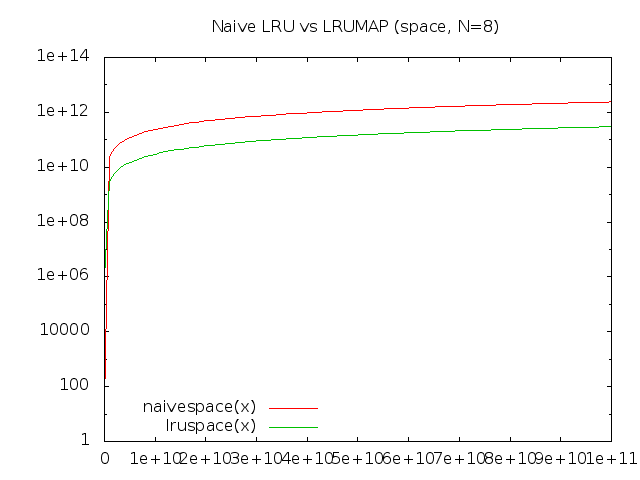
\includegraphics[width=\columnwidth]{out/lrumap8.pdf}
	\caption{Eighth-order LRU}
\label{fig:lru8}
\end{center}
\end{figure}

LRUMAP is even more effective at fourth order, requiring less space than LRU
for all but trivially small $n$ (see Figure ~\ref{fig:lru4}).

\begin{figure}[h]
\begin{center}
	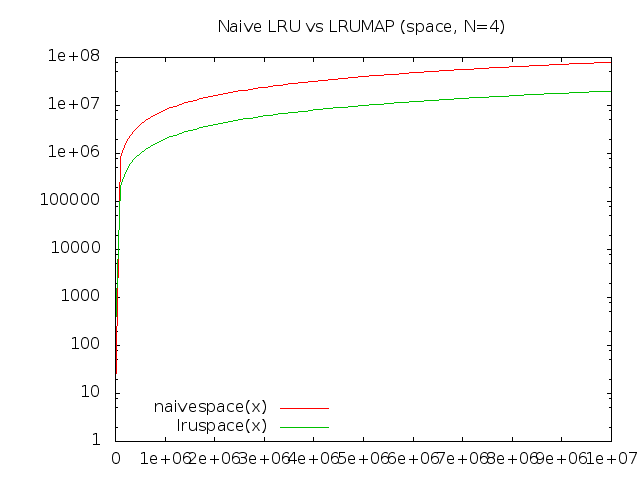
\includegraphics[width=\columnwidth]{out/lrumap4.pdf}
	\caption{Fourth-order LRU}
\label{fig:lru4}
\end{center}
\end{figure}

\section{Beyond LRUMAP}
\subsection{Optimizations}
It may not be necessary to perform true, precise LRU. An entire family of
schemes have been presented, approximating LRU in less time and/or space.
VIA C3\textsuperscript{\textregistered} and Intel processors of the Pentium\textsuperscript{\textregistered} era\citep{shanley} made use of
\textit{pseudo-LRU}, a direction vector-based scheme which requires only
$O(\lg{r})$ bits per set\citep{handy}. The PA-RISC 8600\citep{hurd} likewise used
a proprietary \textit{quasi-LRU} algorithm, with a similar reduction in bits
per set. These schemes can be straightforwardly combined with LRUMAP to yield a
new variant, wherein the LRUMAP entries represent and map among these
algorithms' direction vectors rather than an order's permutations. There seems
no advantage in doing so, however; Pseudo-LRUMAP will consume strictly more space
than Pseudo-LRU, and is unlikely to provide a speed advantage.

A direction vector is $\lg{r}$ bits, and the set of direction vectors is thus
composed of $2^{\lg{r}}=r$ members. Just as before, we precompute a constant
table, this time containing $r \lg{r}$-bit transitions for each of $r$
entries. Each of $n$ sets will require a $\lg{r}$-bit encoding of its current
pseudo-LRU state. A single operation still suffices to update the metastate.
Again allowing for $p$ updates in parallel, we derive Table ~\ref{tab:plru}.

\begin{table}[h]
\begin{center}
	\begin{tabular}{|l|l|l|}
	\hline
	& Pseudo-LRU & Pseudo-LRUMAP \\
	\hline
	Time & $O(\lceil\frac{\lg{r}}{p}\rceil), {p}\le{\lg{r}}$ & $O(1)$ \\
	\hline
	Space & $O(n\lg{r})$ & $O(r^{2}\lg{r}) + O(n\lg{r})$ \\
	\hline
	\end{tabular}
	\caption{Essential properties of Pseudo-LRU/LRUMAP}
\label{tab:plru}
\end{center}
\end{table}

In this case, however, the updates being performed involve $\lg{r}$ single bits.
We've assumed $r$ to be less than or equal to 8; even an 8-bit embedded processor
could thus perform the updates in parallel. Pseudo-LRUMAP cannot be expected to
provide any improvement over Pseudo-LRU.
\subsection{Extensions}
It is trivial to adapt LRUMAP to the Most-Recently-Used methodology, employed
by page caches when a ``looping sequential''\citep{dewitt} access pattern is
detected.
\section{Related Work}
\textbf{WRITE ME! -- JOLENE}
\bibliographystyle{abbrvnat}
\bibliography{cs7260final}
\end{document}
